Esta fase se refiere a explorar la \hyperlink{abbr}{BD} para extraer información
necesaria para poder convertirla en elementos que permitan a un algoritmo
extraer información y aprender de ellos.

Se estudia cada atributo y sus características: tipo de dato (entero, flotante,
booleano), datos y valores faltantes así como su porcentaje, ruido (estocástico,
errores de redondeo), tipo de distribución de probabilidad (gaussiana, uniforme).

Al terminar esta fase estaremos familiarizados con los datos, lo cual nos
permitirá diseñar los algoritmos de preprocesamiento para poder alimentar los
modelos que probaremos en las fases subsecuentes. Al realizar bien esta fase, en
especial la documentación, podremos realizar iteraciones con mayor velocidad y
facilidad, lo cual nos permitirá enfocarnos en la solución y no en su búsqueda.

\subsection{Análisis de atributos}

En \hyperlink{abbr}{ML} se utilizan datos tabulares para realizar el aprendizaje
en donde cada fila representa una muestra y cada columna representa un atributo.
Las columnas en un archivo tabular se dividen en dos: atributos y etiqueta.
Donde el atributo son los valores de las variables de decisión y la etiqueta es
la clase a la que pertenece cada muestra\footnote{En casos de regresión, en
lugar de etiquetas serían valores continuos.}.

\subsubsection{Atributos para la clasificación}

Las columnas ID y Class se refieren al nombre del archivo de cada imagen y a la
clase a la que pertenece. Las demás corresponden a las características extraídas
mediante algoritmos de \hyperlink{abbr}{PDI} para posteriormente ser alimentadas
a algún algoritmo que trabaje con datos tabulares (\autoref{tabla:columnas}).

No todos los atributos de una base de datos se pueden utilizar o son
utilizables, por eso se crea un subconjunto donde se excluyen los atributos que
no se utilizarán para la inferencia o entrenamiento. En este caso los atributos
importantes ya fueron pre-seleccionados.

\begin{table}[H]
    \centering
    \resizebox{0.4\textwidth}{!}{%
    \begin{tabular}{@{}ll@{}}
    \toprule
    Columna & Característica \\ \midrule
    Kerne\_A & Área del núcleo \\
    Cyto\_A & Área del citoplasma \\
    K/C & Proporción N/C \\
    Kerne\_Ycol & Brillo del núcleo \\
    Cyto\_Ycol & Brillo del citoplasma \\
    KerneShort & Diámetro corto del núcleo \\
    KerneLong & Diámetro largo del núcleo \\
    KerneElong & Elongación del núcleo \\
    KerneRund & Redondez del núcleo \\
    CytoShort & Diámetro corto del citoplasma \\
    CytoLong & Diámetro largo del citoplasma \\
    CytoElong & Elongación del citoplasma \\
    CytoRund & Redondez del citoplasma \\
    KernePeri & Perímetro del núcleo \\
    CytoPeri & Perímetro del citoplasma \\
    KernePos & Posición relativa del núcleo \\
    KerneMax & Máximo en núcleo \\
    KerneMin & Mínimo en núcleo \\
    CytoMax & Máximo en citoplasma \\
    CytoMin & Mínimo en citoplasma \\ \bottomrule
    \end{tabular}%
    }
    \caption{Columnas del archivo y la característica que representa}\label{tabla:columnas}
    \end{table}

\subsubsection{Conteo de clases y categorías}

Los resultados del análisis exploratorio de datos se encuentran en
la~\autoref{tabla:exploratorio}. Los datos se encuentran desbalanceados por lo
que se tendrán que generar políticas para balancearlos tanto en clase como
categoría, dentro de estos algoritmos también se estandarizará el tamaño de las
imágenes puesto que estas varían en tamaño (\autoref{tabla:dimensiones}).

\begin{table}[H]
    \centering
    \resizebox{\textwidth}{!}{%
    \begin{tabular}{@{}lllll@{}}
    \toprule
    Clase & Categoría & Tipo & Cantidad & Subtotales \\ \midrule
    0 & Normal & Superficial squamous epithelial & 74 &  \\
    1 & Normal & Intermediate squamous epithelial & 70 &  \\
    2 & Normal & Columnar epithelial & 98 & 242 normales \\ \midrule
    3 & Anormal & Mild squamous non-keratinizing dysplasia & 182 &  \\
    4 & Anormal & Moderate squamous non-keratinizing dysplasia & 146 &  \\
    5 & Anormal & Severe squamous non-keratinizing dysplasia & 197 &  \\
    6 & Anormal & Squamous cell carcinoma in situ intermediate & 150 & 675 anormales \\ \bottomrule
    \end{tabular}%
    }
    \caption{Resultados del análisis exploratorio de datos de la base de datos de entrenamiento}\label{tabla:exploratorio}
    \end{table}
 
\begin{table}[H]
    \centering
    \resizebox{0.3\textwidth}{!}{%
    \begin{tabular}{lll}
     & Altura & Ancho \\
    Promedio & 139.73 & 155.65 \\
    Máximo & 439 & 768 \\
    Mínimo & 32 & 40
    \end{tabular}%
    }
    \caption{Análisis de dimensiones}\label{tabla:dimensiones}
    \end{table}

\subsubsection{Análisis de dato individual}

No solo se encuentran imágenes de las células en la \hyperlink{abbr}{BD}, sino
también imágenes que son máscaras para determinar como se segmentan las partes
de la célula en la imagen: núcleo, citoplasma y fondo. Estas máscaras
corresponden a imágenes representadas por una sola matriz. Esta segmentación fue
realizada por expertos cito-tecnólogos utilizando software
especializado\footnote{Las imágenes fueron clasificadas y validadas por un
conjunto de expertos, si alguno discrepaba en la clasificación, la imagen se
eliminaba.}~(\autoref{fig:imagen_mascara}).

\begin{figure}[H]
    \centering
    \begin{subfigure}{.5\textwidth}
        \centering
        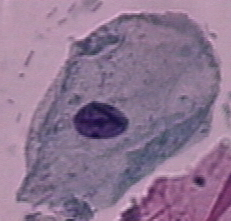
\includegraphics[width=.8\linewidth]{capitulo_sdac/209522940-209523052-001}
        \caption{Imagen}
    \end{subfigure}%
    \begin{subfigure}{.5\textwidth}
        \centering
        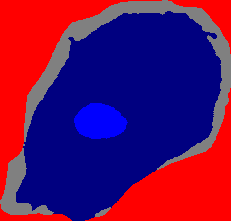
\includegraphics[width=.8\linewidth]{capitulo_sdac/209522940-209523052-001-d}
        \caption{Máscara}
    \end{subfigure}
    \caption{Imagen de célula y su máscara segmentada}\label{fig:imagen_mascara}
    \end{figure}

\subsection{Aplicar estadísticas}

Aquí se exploran las características numéricas de las datos que componen la base
de datos, por ejemplo, el número de elementos faltantes por columna. Estudiar
correlaciones entre los atributos nos permite determinar si estamos trabajando
bajo un sistema lineal o no lineal. Esto es importante debido a que uno no puede
ajustar un modelo lineal a datos no lineales, pero tampoco se puede ajustar un
modelo no lineal a datos lineales. 

\subsubsection{Análisis de correlación}

Para esta tesis no es necesario aplicar estadísticas a los atributos ya que
usaremos imágenes, esta es la ventaja del uso de \hyperlink{abbr}{DL} por sobre
otras técnicas de \hyperlink{abbr}{ML}. Se deja la gráfica de correlación entre
los atributos como ejemplo en la \autoref{fig:correlacion}.

\begin{figure}[H]
\centering
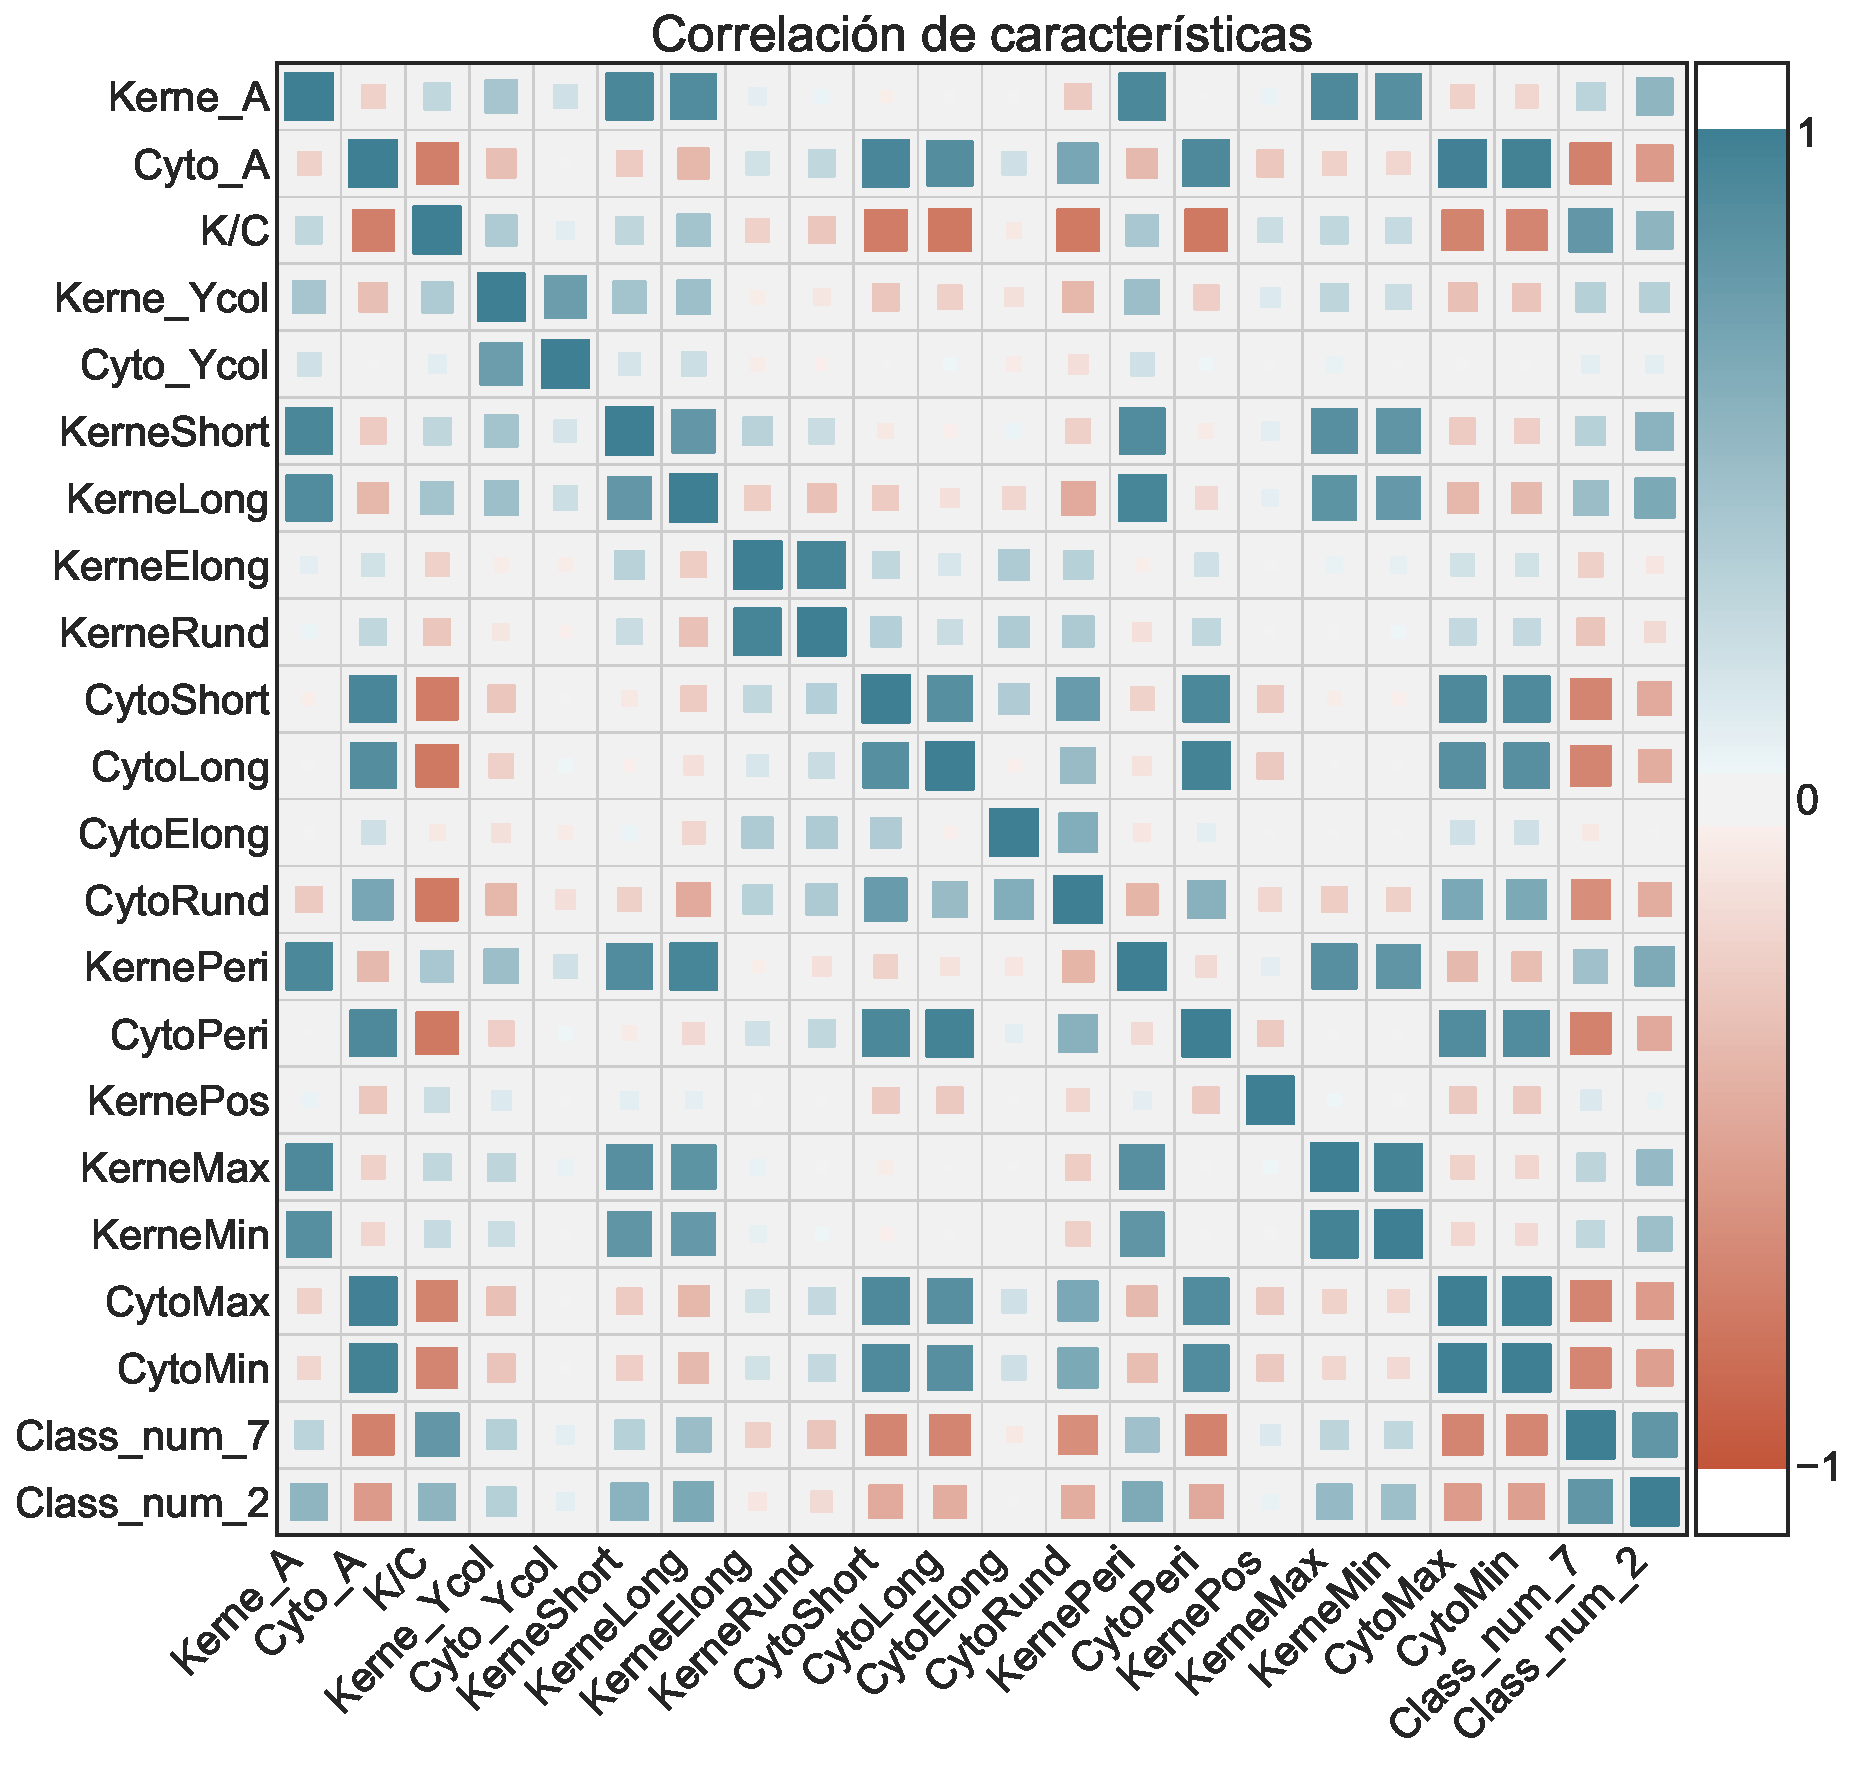
\includegraphics[width=0.8\textwidth]{capitulo_sdac/correlacion}
\caption{Correlación entre características del archivo}\label{fig:correlacion}
\end{figure}

\subsection{Visualización}

Visualizar no solo significa generar muestras, si trabajamos con datos
tabulares, en especial aquellos con muchas columnas donde es difícil graficar
debido a que cada columna representa una dimensión; visualizar significa también
aplicar algoritmos de reducción de dimensionalidad como PCA para poder graficar
en dos dimensiones lo que antes tenia muchas más.

\subsubsection{Muestras}

Procedemos a analizar las muestras en las \autoref{fig:muestras_celulas} y en
\autoref{fig:muestras_mascaras}. Donde observamos siete muestras por cada una de
las siete clases, cada fila representa una clase distinta. Podemos observar
claramente algunas características morfológicas que dan indicios de porque se
eligieron algunas de estas para entrenar algoritmos de clasificación.

Salta a la vista el tamaño del núcleo entre las categorías normales y anormales.
También podemos ver que las células columnares, aunque son normales, comparten
morfología con las anormales. Es por ello que generamos el supuesto de que el
núcleo celular tiene suficiente información para clasificar las células entre
sus clases y categorías. Las muestras de las máscaras consisten en otro muestreo
aleatorio, aquí también podemos ver que el tamaño y morfología del núcleo son
cruciales para clasificar las células.

\begin{figure}[]
    \centering
    \includegraphics[width=1\textwidth]{capitulo_sdac/muestras_celulas}
    \caption{Muestreo de la BD}\label{fig:muestras_celulas}
\end{figure}

\begin{figure}[]
    \centering
    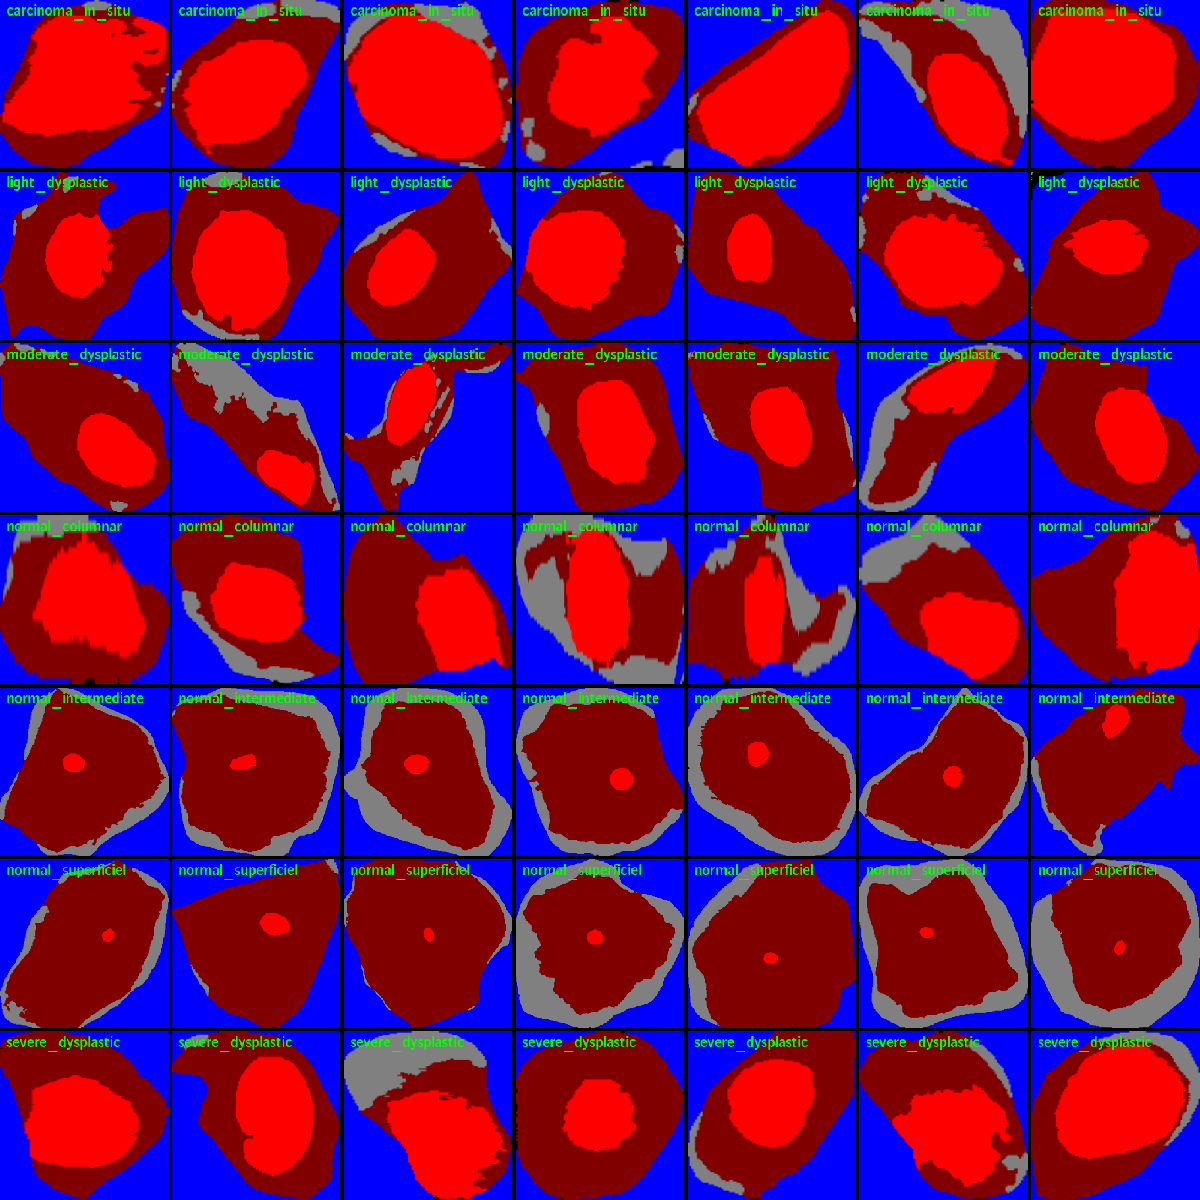
\includegraphics[width=1\textwidth]{capitulo_sdac/muestras_mascaras}
    \caption{Muestreo de la BD}\label{fig:muestras_mascaras}
\end{figure}

\subsection{Identificar transformaciones}

En esta esta debemos identificar transformación aplicables: Estas
transformaciones pueden incluir transposición matricial, cambio de espacio de
color, cambio en la escala de tiempo, etcétera.

Para datos tabulares, se pueden aplicar transformaciones para cambiar la escala
de los datos y restringirlos a valores pequeños para facilitar el aprendizaje
del modelo. Normalizar se refiere a restringir los datos a una escala entre 0 y
1. Estandarizar resta la media y divide por la varianza.

\subsubsection{Transformaciones aplicables a imágenes}

Transformaciones en imágenes incluyen normalizar pixeles a un rango entre 0 y 1, dividiendo
entre 255 la intensidad de cada pixel (\autoref{eq:pixel_norm}).

\begin{equation}
    \label{eq:pixel_norm}
    I_{norm} = I_{p} / 255
\end{equation}

En nuestro caso, las imágenes celulares tienen dos tipos de simetría. La
simetría axial es, dado cierto eje, podemos reflejar la imagen y seguirá siendo
simétrica. La simetría radial, es dado un punto, podremos rotar la imagen sobre
él sin que pierda su propiedad de simetría.

\begin{figure}[H]
    \centering
    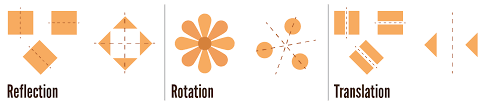
\includegraphics[width=0.7\textwidth]{capitulo_sdac/simetrias}
    \caption{Tipos de simetría}\label{fig:simetrias}
\end{figure}

La normalización nos ayudará a entrenar la \hyperlink{abbr}{ConvNet}, reduciendo la libertad de
valores que puede tomar cada peso dentro de la red. Mientras que las
transformaciones de simetría nos ayudarán en la fase de aumento para generar más
datos e incrementar el poder de generalización del modelo.

\subsection{Información}

Al finalizar este proceso, habremos generado información pertinente que nos
ayudará a pre-procesar los datos para su posterior entrenamiento. Sabemos
cuantos datos tenemos y de que clase, información estadística de la \hyperlink{abbr}{BD}, como
es cada dato individual y las transformaciones que se le pueden aplicar al mismo.

Ya que la imagen contiene la célula y su máscara, pero no contiene las
coordenadas de cada objeto dentro de la imagen o imágenes con múltiples objetos,
podremos aplicar clasificación y segmentación semántica pero no detección ni
instanciación. Esto nos da un indicio de los algoritmos y arquitecturas a utilizar.

Finalmente, aumentaremos el archivo de excel que encontramos dentro de la
carpeta de la \hyperlink{abbr}{BD} de la siguiente manera
(\autoref{tabla:ananidas}). Este archivo servirá como inicio para los algoritmos
posteriores de pre-procesamiento. 

% Please add the following required packages to your document preamble:
% \usepackage{booktabs}
% \usepackage{graphicx}
\begin{table}[H]
    \centering
    \resizebox{0.5\textwidth}{!}{%
    \begin{tabular}{@{}ll@{}}
    \toprule
    Columna & Descripcion \\ \midrule
    Class\_cat\_2 & Clase categórica binaria \\
    Class\_num\_2 & Clase numérica binaria \\
    Class\_cat\_7 & Clase categórica multi-clase \\
    Class\_num\_7 & Clase numérica multi-clase \\
    file & Dirección absoluta de la imagen \\
    file\_masks & Dirección absoluta de la máscara \\ \bottomrule
    \end{tabular}%
    }
    \caption{Columnas añadidas al archivo}\label{tabla:ananidas}
    \end{table}

